\documentclass[12pt,a4paper]{article}

\usepackage{fancyhdr}
\usepackage{lastpage}
\usepackage{amsthm}
% \usepackage[sorting=none]{biblatex}
\usepackage{hyperref}
\usepackage{amsmath}
\usepackage{amsfonts}
\usepackage{siunitx}
\usepackage{mathabx}
\usepackage[inkscapelatex=false]{svg}
\usepackage{footnote}
\usepackage{tablefootnote}
\usepackage{makecell}
\usepackage[letterpaper, left=2cm,right=2cm,top=3cm,bottom=2cm]{geometry}
\usepackage{longtable}
\usepackage{multirow}
\usepackage{array}
\usepackage{verbatim}
\usepackage{minted}
\usepackage{booktabs}
\usepackage{algorithm}
\usepackage{algpseudocode}
\usepackage{subcaption}
\usepackage{graphicx}
\usepackage{subfigure}
\usepackage[toc,page]{appendix}
\usepackage[version=4]{mhchem}
\usepackage{setspace}
\usepackage{placeins}
\usepackage{wrapfig}
\usepackage{csquotes}
\usepackage[style=authoryear-ibid,backend=biber]{biblatex}
\addbibresource{EPQ.bib}

% layout
\pagestyle{fancy}
\fancyhf{}
\rhead{Page \thepage\ of \pageref*{LastPage}}
\fancyfoot[C]{\thepage}
\setlength{\headheight}{14.5pt}
\setlength{\parindent}{0pt}
\setlength{\parindent}{0em}

% title
\author{Chenyu Shi}
\date{}
\title{\Huge{\bf{\ntitle}}}

% Others

\hypersetup{
  colorlinks=true,
  urlcolor=blue,
  linkcolor=red,
  citecolor=black
}

%%%%%%%%%%%%%%%%%%%%%%%%%%
%%%%%%%%%% math %%%%%%%%%%
%%%%%%%%%%%%%%%%%%%%%%%%%%

% Theorems
\theoremstyle{definition}
\newtheorem{thm}{Theorem}[section]
\newtheorem{axiom}[thm]{Axiom}
\newtheorem{conjecture}[thm]{Conjecture}
\newtheorem{cor}[thm]{Corollary}
\newtheorem{defi}[thm]{Definition}
\newtheorem{eg}[thm]{Example}
\newtheorem{lemma}[thm]{Lemma}
\newtheorem{notation}[thm]{Notation}
\newtheorem{prop}[thm]{Proposition}

\newtheorem{question}{Question}

\newtheorem*{aim}{Aim}
\newtheorem*{assumption}{Assumption}
\newtheorem*{claim}{Claim}
\newtheorem*{ex}{Exercise}
\newtheorem*{fact}{Fact}
\newtheorem*{law}{Law}
\newtheorem*{remark}{Remark}
\newtheorem*{rrule}{Rule}
\newtheorem*{warning}{Warning}



\newenvironment{solution}{\begin{proof}[Solution]}{\end{proof}}

% Special sets
\newcommand{\C}{\mathbf{C}}
\newcommand{\R}{\mathbf{R}}
\newcommand{\Q}{\mathbf{Q}}
\newcommand{\Z}{\mathbf{Z}}
\newcommand{\N}{\mathbf{N}}
\newcommand{\F}{\mathbf{F}}
\setlength{\parindent}{0em}
% Symbols
\newcommand{\abs}[1]{\left\lvert #1\right\rvert}
\newcommand{\floor}[1]{\left\lfloor #1\right\rfloor}
\newcommand{\ceil}[1]{\left\lceil #1\right\rceil}
\newcommand{\set}[1]{\{#1\}}
\newcommand{\limit}[2]{\lim\limits_{#1\to #2}}
\renewcommand{\d}{\mathop{}\!\mathrm{d}} 
\renewcommand{\vec}[1]{\boldsymbol{\mathbf{#1}}}
\renewcommand{\P}{\mathrm{P}}
\DeclareMathOperator{\lcm}{lcm}
\DeclareMathOperator{\E}{E}
\DeclareMathOperator{\Var}{Var}

\begin{document}
    \epqtitle
    \newpage
    \tableofcontents    
    \newpage  
    \setstretch{2}
    \setlength{\parindent}{2em}
    
    \section{Abstract}
    This study rigorously examines the role of carbon dioxide (\ce{CO2}) emissions in influencing global warming and their impacts on the environment and human society. Through a detailed literature review, the paper elucidates the dual nature of \ce{CO2} as both a vital component of the Earth's carbon cycle and a significant contributor to the greenhouse effect, which exacerbates global warming. Employing polynomial fitting and autoregressive integrated moving average (ARIMA) models, the research quantitatively predicts future \ce{CO2} emission trends, projecting a significant increase in atmospheric \ce{CO2} concentrations over the next few decades. Additionally, the study explores the correlation between \ce{CO2} emissions and global temperature rise through covariance and linear regression analysis, establishing a strong positive relationship. The findings highlight the urgent need for effective strategies and policies to mitigate \ce{CO2} emissions and address the challenges of global warming. This paper contributes to the ongoing discourse on environmental management, offering insights that can inform future research, policy development, and global efforts towards sustainability and climate change mitigation.

    \section{Introduction}
    \subsection{Background Information}
    Carbon dioxide (\ce{CO2}), which comprises approximately $0.04\%$ of the Earth's atmosphere, plays a pivotal role in both sustaining life and influencing the planet's climate. Produced through the combustion of organic substance and the respiration of living organisms, \ce{CO2} is intricately linked to life on Earth. As for the industrial aspect, it emerges as a predominant byproduct of combustion processes.

    The duality of \ce{CO2}'s role is stark. On one hand, it is essential for the carbon cycle and plant photosynthesis, underpinning the existence of life. On the other, as a greenhouse gas, it traps heat in the atmosphere, contributing significantly to global warming. This phenomenon poses a long-discussed threat, potentially leading to catastrophic environmental changes such as rising sea levels, ice melt, and altered climates. The consensus is that human activities are the principal contributors to \ce{CO2} emissions, thereby exacerbating global warming.

    Over recent decades, a rapid increase in \ce{CO2} emissions has paralleled escalating global warming concerns. The ensuing environmental challenges threaten terrestrial life, compelling humanity to seek strategies for reducing \ce{CO2} emissions and mitigating global warming's impacts. This paper endeavors to quantitatively assess the effects of \ce{CO2} emissions on global warming, aiming to highlight the urgent need for environmental stewardship and emissions reduction.

    \subsection{Report Structure}
    This report comprises a literature review that synthesizes previous studies on \ce{CO2} emissions and global warming, providing a comprehensive overview of the subject, including the impacts of emissions and human responses. Following this, I will present predictions of future \ce{CO2} emissions using methods including polynomial fitting and an autoregressive integrated moving average (ARIMA) model. Additionally, the relationship between \ce{CO2} emissions and global warming will be examined through covariance and linear regression models. The discussion will interpret the results and implications of these predictions and analyses, acknowledging the methods' limitations and presenting recommendations for future studies.
        
    \section{Literature Review}
    \subsection{Introduction}
    This section offers a comprehensive overview of the project by referencing previous studies to introduce the broader impact of \ce{CO2}. Firstly, I will investigate the current \ce{CO2} emission condition by analyzing ppm values and other factors with specific annual data. Secondly, I will explore the influences of \ce{CO2} emission across ecosystem and human society. Finally, I will focus on elaborating human's response to \ce{CO2} emission, including actions of organizations and nations.
    
    \subsection{Emission Condition}
    
    Before the Industrial Revolution, the concentration of \ce{CO2} in atmosphere was approximately $280$ parts per million (abbr. ppm in the following) \autocite{neftel_evidence_1985}. The value exploded to $377.7$ ppm in 2004, a striking rise of roughly $35\%$ \autocite{pieter_t_trends_2022}. More surprisingly, according to researchers from National Oceanographic and Atmospheric Administration and Scripps Institution of Oceanography, the monthly mean \ce{CO2} concentration level peaked at $421$ ppm in May 2022, which reflected an increasingly serious condition at present \autocite{national_oceanographic_and_atmospheric_administration_carbon_2022}. Additionally, an Organisation for Economic Co-Operations and Development report predicts a \ce{CO2} level of $685$ ppm by 2050, indicating that the prospect of dealing with \ce{CO2} emission is not optimistic \autocite{organisation_for_economic_co-operations_and_development_oecd_2012}.

    As for specific average \ce{CO2} emission changed annually, measurements from Mauna Loa Observatory are listed in \hyperref[emission]{Table \ref*{emission}} and visualized in \hyperref[emission_line]{Figure \ref*{emission_line}}, in which we can observe the steady increase of the amount of \ce{CO2} emission \autocite{national_oceanographic_and_atmospheric_administration_gml_data_notitle_2023}.
    \begin{figure}[htbp]
        \centering
        \captionof{table}{Average \ce{CO2} emission annually}
        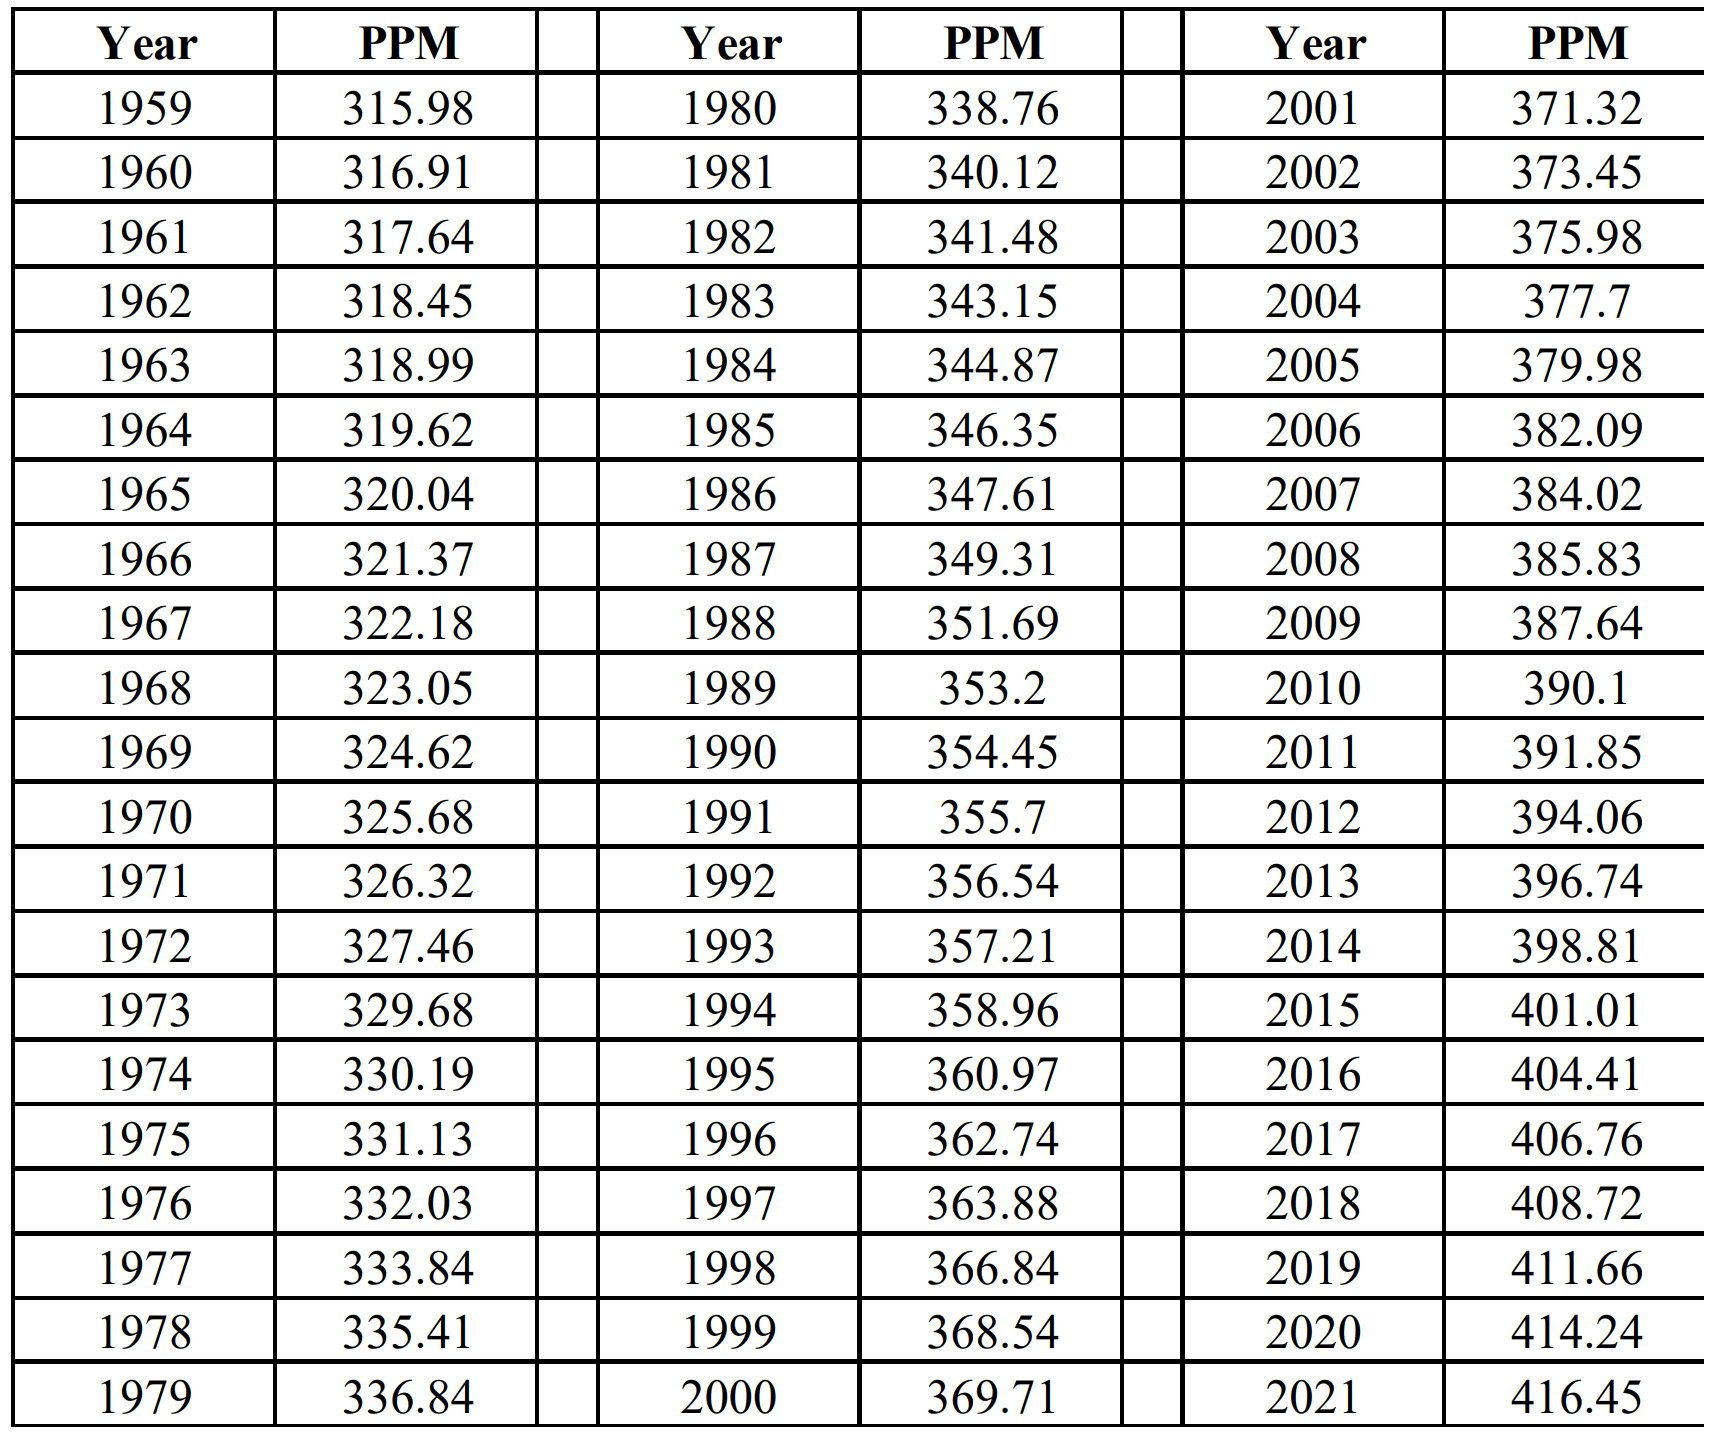
\includegraphics[width=\linewidth]{img/emission.png}
        \label{emission}
    \end{figure}
    \begin{figure}[htbp]
        \centering
        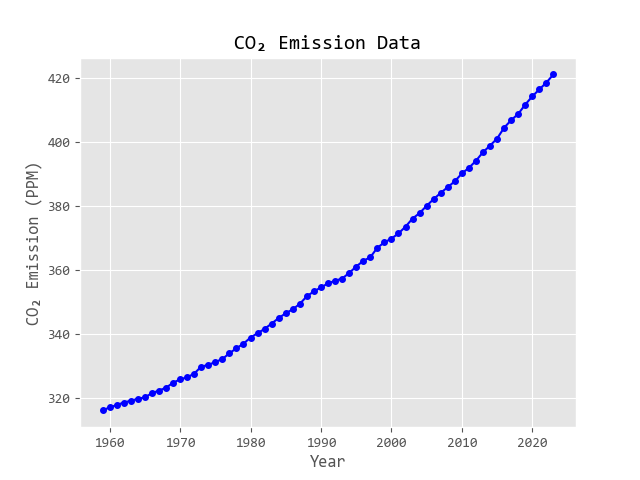
\includegraphics[width=0.5\linewidth]{img/emission_line.png}
        \caption{\ce{CO2} emission Graph}
        \label{emission_line}
    \end{figure}
    
    Apart from ppm value as elaborated above, there are other aspects discribing the emissions of \ce{CO2} which is quite worth noting. As International Energy Agency reports, in 2022, the emission growth is mainly caused by extreme weather which brings more need for cooling and heating. Despite that, it is reported that industrial emissions declined by $1.7\%$, driven by a reduction in cement and steel production in China. A piece of good news would be the unprecedented advancement of new energy technology, including solar PV and wind energy, which reduce the \ce{CO2} emissions to some extent \autocite{iea_co2_2023}.
    
    \subsection{Effects}
    \subsubsection{Growth of Plants}
    As expected, \ce{CO2} does play an irreplaceable role in stimulating overall biomass of plants, together with increasing the soil C:N ratio and microbial \ce{N} contents \autocite{de_graaff_interactions_2006}. At the same time, it is widely acknowledged and verified by many studies that the increase of atmospheric \ce{CO2} concentrations also leads to the global photosynthesis rise \autocite{campbell_effects_1988,kramer_carbon_1981,qide_effects_1992}. Other benefits of \ce{CO2} include higher plant water use efficiency due to reduction in transpiration, which results in less water comsumption \autocite{prior_review_2011}. Nevertheless, \ce{CO2} may inhibit plant growth to some extent. For instance, higher \ce{CO2} concentration may bring about reduction of concentrations of crucial nutrients such as nitrogen, phosphorus and protein \autocite{conroy_influence_1992}.
    \subsubsection{Global Warming}
    As one of the greenhouse gases, \ce{CO2} is widely being considered as the main driving factor that causes the phenomenon of global warming. Specifically, when the surface of earth automatically dissipate heat to the space in the form of electromagnetic waves, \ce{CO2} can serve to absorb a certain wavelength range of those waves. In this way, it can help trap heat obtained from the sunlight and thus increase global temperature \autocite{seim_influence_2020}. Scientists have found the positive correlation, or even a simple near-linear relation, between \ce{CO2} and global temperature \autocite{matthews_proportionality_2009}.

    Furthermore, global warming has led to considerable serious consequences in many different facets of life on Earth. On climates, increasing \ce{CO2} concentration contributes to more precipitation at a rate of about $7\%$ per kelvin \autocite{lambert_how_2008,stephens_controls_2008,wentz_how_2007}. However, what is more lethal is that by changing large-scale atmospheric circulation patterns, the growing atmospheric \ce{CO2} levels may change the precipitation patterns, that is, make wet place wetter and dry places drier \autocite{national_geographic_society_influence_2023}. As a result, as simulated and measured by several models, the increased frequency and intensity of heavy precipitation, along with the melting of glaciers and polar ice caps, has lead to more severe flooding, which will undoubtedly cause catastrophic consequences \autocite{alfieri_global_2015,alifu_enhancement_2022}. Simultaneously, the level of drought in specific areas increased substantially and will thus bring about large threats to environment and ecosystem \autocite{dai_drought_2011,zeng_increased_2023}. Apart from drought and flooding, many other extreme weather events, including hurricanes and wildfires, also occur more frequently and intensively, under the rising levels of global warming and \ce{CO2} concentration \autocite{anthes_hurricanes_2006,moore_quantifying_2015,torn_predicting_1992}.
    \subsubsection{Ocean Acidification}
    As we all know from the chemical knowledge that the carbon dioxide can react with water to produce carbonic acid, when absorbing excess \ce{CO2} gas, the ocean water is gradually acidified, i.e. its pH value gradually decreases. Numerous studies have revealed that the rate of acidification is progressively increasing, especially as we've entered the 21\textsuperscript{st} century \autocite{doney_ocean_2009,zeebe_history_2012}. We need to recognize as well that the acidification of seawater would have devastating effects to a broad range of marine organisms \autocite{guinotte_ocean_2008}. Specifically speaking, ocean acidification may lead to sensory deficits in marine organisms and have a negative impact on several physiological processes such as respiration, reproduction and excretion, which thus increases their general death rate \autocite{gazeau_impacts_2013,kroeker_impacts_2013,radford_ocean_2021}. For instance, coral reefs are highly susceptible to ocean acidification due to their predominant composition of \ce{CaCO3} which is likely to dissolve in acidic water, and the consequently increasing dissolution rate and reducing calcification rate pose a significant threat to the growth of coral reefs \autocite{kleypas_coral_2009,silverman_coral_2009}. 
    \subsubsection{Ecosystem}
    Generally speaking, the elevated concentration of \ce{CO2} inflicts substantial harm on the Earth's ecosystem. As analyzed above, the rapid increase of \ce{CO2} concentration with cause dramatic change of global climate and environment, which will have a wide impact on the distribution and behavior of plant and animal species, many of wh ich may suffer a rise in mortality. Thereinto, changes in the number of key species can have cascading effects throughout food webs \autocite{schindler_influence_1997}. That means, some species may be affected indirectly due to the change of their predators or food source, which can bring about an imbalance in ecosystem. At the same time, the survival of a number of species, particularly those that are less resilient to rapid environmental change, are greatly threatened under change of \ce{CO2} concentration, implying shifts in the composition and structure of ecosystem and loss of biodiversity \autocite{korner_biodiversity_1995}.
    \subsubsection{Mankind}
    In addition to environmental influence, the impact of elevated \ce{CO2} concentration on human beings is also noteworthy. In agricultural aspect, while it is true that extreme weathers like drought may contribute to a decline in crop yield \autocite{sun_does_2023}, it is found that the promoting effect of \ce{CO2} to plant growth outweighs its harm, that is to say, in general, the crop yield is positively correlated to the concentration of \ce{CO2} within a certain range \autocite{yang_rice_2024}.

    Regarding human health, firstly, it has been found that the growing \ce{CO2} concentration can have adverse effects on the nutrient content in food, specifically a decline of $5\%$ to $15\%$ in protein and mineral concentrations and even up to $30\%$ in B vitamins \autocite{loladze_hidden_2014,myers_increasing_2014,zhu_carbon_2018}. On top of that, research indicates that elevations in ambient \ce{CO2} would pose direct risks for human health, resulting in potential health problems including inflammation, bone demineralization and endothelial dysfunction among others \autocite{jacobson_direct_2019}.
    
    \subsection{Human's response}
    Confronted with such pressing issue, many organizations have made great efforts to inhibit the increase of \ce{CO2} concentration. For example, in Katowice Climate Change Conference, 15 international organizations, including United Nations Framework Convention on Climate Change (UNFCCC), have made their announcements of reducing carbon emmissions to make climate neutral by actions of installing solar photovoltaic systems and efficient cooling systems, reducing air travel and so on \autocite{unfccc_15_2018}. Nations are taking actions as well. Take China as an example, it has made targets to reach peak carbon emissions by 2030 and achieve carbon neutrality by 2060 \autocite{xinhua_responding_2021}.
    
    \subsection{Conclusion}
    To conclude, currently, \ce{CO2} emissions have increased significantly compared with pre-industrial times and are steadily rising annually. While elevated levels of \ce{CO2} can promote plant growth, it may also bring about catastrophes such as global warming and ocean acidification. As a result, the global climates are disrupted and extreme weather events are more frequent. It may then threaten the survival of animals and plants, thereby jeopardizing biodiversity and harming sustainability. As for human, though rising \ce{CO2} concentration helps with the algriculture development to some extent, unfortunately, studies reveal that it may pose considerable potential health problems for human beings. Therefore, organizations and nations have made plans to reduce carbon emission, and people are pulling together to address the problem by means like developing renewable energy sources.

    \section{Prediction}
    \subsection{Introduction}
    As mentioned above, the emission of \ce{CO2} has greatly influence the life in earth as well as human society. Therefore, the prediction of \ce{CO2} emission is of great importance to help people to make decisions and take actions to reduce the emission of \ce{CO2}. In this section, based on the data in \hyperref[emission]{Table \ref*{emission}}, I will use two methods, polynomial fitting and ARIMA model, to predict the future \ce{CO2} emission.
    \subsection{Methodology}
    \subsubsection{Polynomial Fitting}
    Polynomial fitting is a basic method to fit a curve to a set of data points. It is a simple and intuitive method to predict the future \ce{CO2} emission. The basic idea of polynomial fitting is to find a polynomial function, which is in the form of $f(x)=a_nx^n+a_{n-1}x^{n-1}+\cdots+a_1x+a_0$, that fits the data points. We notice that in order to use the polynomial function to find the prediction of future emission, we need to use the current measured data, i.e. the data in \hyperref[emission]{Table \ref*{emission}}, to determine the parameters of the polynomial function, including the degree $n$ and the coefficients $a_0,a_1,\dots,a_n$.

    For the degree $n$ of the function, it is determined by the number of data points and the complexity of the data. The degree of the polynomial function should be chosen to balance the accuracy and the complexity of the function. The higher the degree of the polynomial function, the more accurate the prediction will be. However, a higher degree of the polynomial function would have higher complextity, and may also lead to overfitting, which means the function fits the data points too well and focus on the local features of the existing data points too much, and thus may not be able to predict the future data accurately.

    As along as the degree of the polynomial function is determined, we should think about how to find the coefficients $a_0,a_1,\dots,a_n$ such that the function best \textit{fits} the data points. First we need to define a \textit{standard} for fitting, formally speaking, we need to define a \textit{loss function} to measure the difference between the predicted value and the actual value. In this project, we use a common loss function, the least square loss function, which is defined by
    \begin{equation}
        L(a_0,a_1,\dots,a_n)=\sum_{i=1}^m(f(x_i)-y_i)^2
    \end{equation}
    where the data points are $(x_1,y_1),(x_2,y_2),\dots,(x_m,y_m)$.

    Then our goal is to find the coefficients $a_0,a_1,\dots,a_n$ such that the loss function $L(a_0,a_1,\dots,a_n)$ is minimized. Mathematically, this implies for all $i=0,1\dots,n$, we have
    \begin{equation}
        \frac{\partial L}{\partial a_i}=0
    \end{equation}
    which gives us a system of $n+1$ equations to solve for the coefficients $a_0,a_1,\dots,a_n$. This system of equations is called the \textit{normal equation} of the least square loss function. The solution of the normal equation is unique and can be found by linear algebra methods.
    
    Back to the question, we first consider the case of degree $n=1$, i.e. linear fitting. After solving the equation system, we can obtain the linear function
    \begin{equation}
        f(x)=1.6415x-2909.001
    \end{equation}
    as plotted in \hyperref[linear_fitting]{Figure \ref*{linear_fitting}}.
    
    \begin{figure}[htbp]
        \centering
        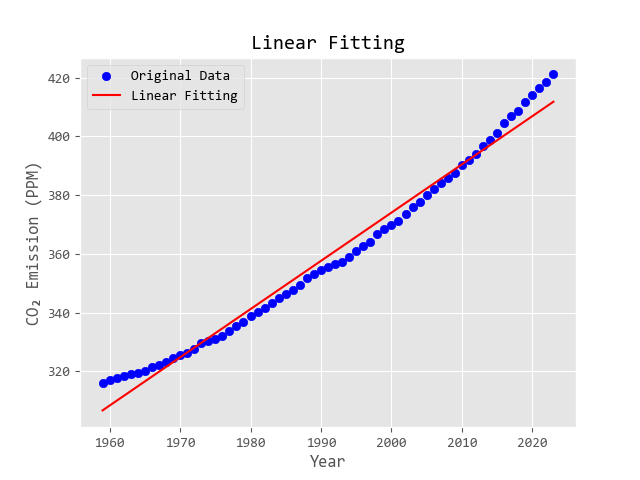
\includegraphics[width=0.5\linewidth]{img/linear fitting.png}
        \caption{Linear Fitting}
        \label{linear_fitting}
    \end{figure}

    In this case, the prediction for \ce{CO2} emission in the year $2030$, $2050$, $2070$ and $2100$ are respectively $423.28$, $456.11$, $488.94$ and $538.18$ PPM. 

    However, we should notice that the linear fitting is not accurate enough, as the actual data points are not linearly distributed. Therefore, we should consider higher degree of polynomial function to fit the data points.

    Then we consider the case of degree 2. After calculation, the function is given by
    \begin{equation}
        f(x)=0.01314x^2-50.6842x+49176.647
    \end{equation}
    as plotted in \hyperref[quadratic_fitting]{Figure \ref*{quadratic_fitting}}.

    \begin{figure}[htbp]
        \centering
        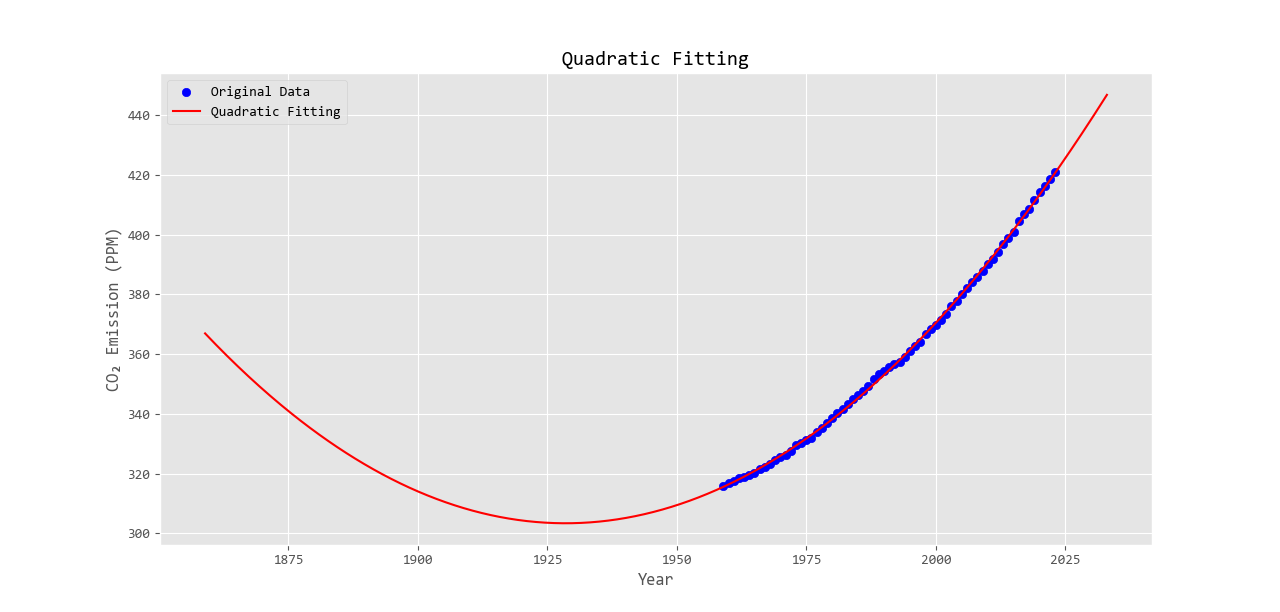
\includegraphics[width=1\linewidth]{img/quadratic fitting.png}
        \caption{Quadratic Fitting}
        \label{quadratic_fitting}
    \end{figure}
    
    In this case, the prediction for \ce{CO2} emission in the year $2030$, $2050$, $2070$ and $2100$ are respectively $438.64$, $497.23$, $566.32$ and $689.68$ PPM.

    We then consider the case of degree 3. After calculation, the $f(x)$ is given by
    \begin{equation}
        f(x)=0.00004x^3-0.22568x^2+424.7802x-266339.62
    \end{equation}
    as plotted in \hyperref[cubic_fitting]{Figure \ref*{cubic_fitting}}.

    \begin{figure}[htbp]
        \centering
        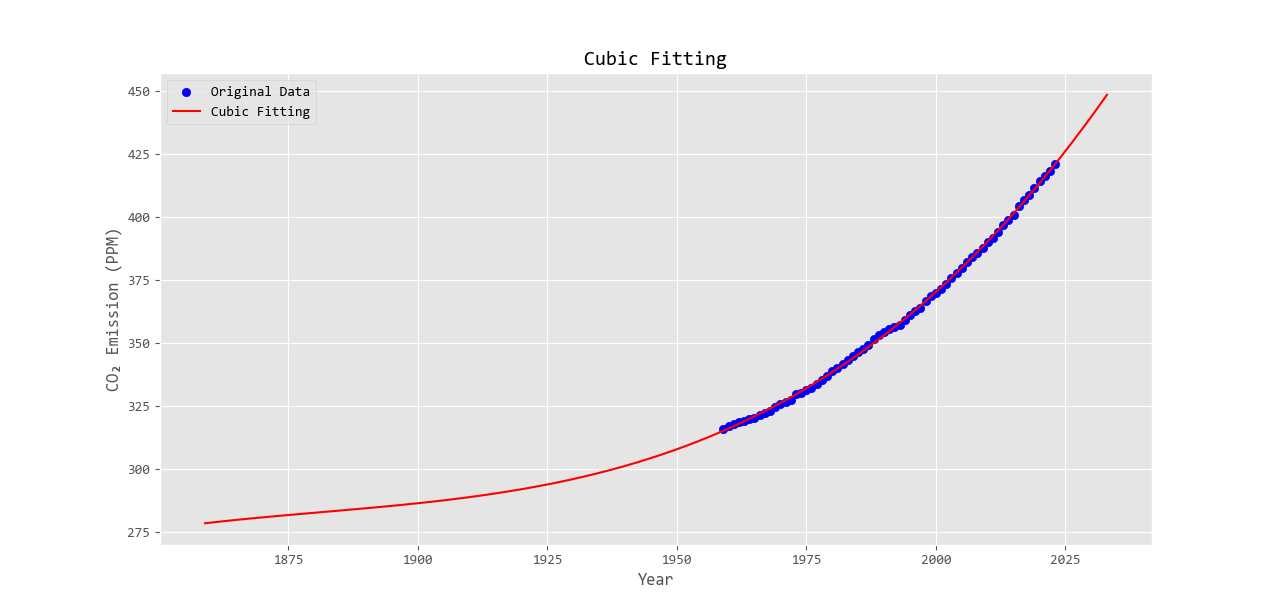
\includegraphics[width=1\linewidth]{img/cubic fitting.png}
        \caption{Cubic Fitting}
        \label{cubic_fitting}
    \end{figure}
    
    In this case, the prediction for \ce{CO2} emission in the year $2030$, $2050$, $2070$ and $2100$ are respectively $440.02$, $503.94$, $584.04$ and $738.70$ PPM.
    
    We notice that the cubic function is already really close to our data points, and the prediction for the future \ce{CO2} emission is already accurate enough. Therefore, we stop here and do not consider higher degree of polynomial function, which may lead to higher complexity and overfitting.
    
    By comparing the prediction of \ce{CO2} emission using polynomial fitting with different degrees, we notice that the prediction of \ce{CO2} emission is increasing, which is consistent with the actual data points. More specifically, we observe that the prediction of \ce{CO2} emission in year $2100$ nearly doubles that in year $2000$, from the more accurate results of quadratic and cubic fitting. This is a clear evidence that the \ce{CO2} emission is increasing and the global warming is becoming more and more serious.
    
    \subsubsection{ARIMA}
    We need to recognize that polynomial fitting has some limitations in the prediction of \ce{CO2} emission. For example, the prediction of \ce{CO2} emission using polynomial fitting is based on the assumption that the future \ce{CO2} emission will follow the same pattern as the past \ce{CO2} emission. However, this assumption may not be true, as the future \ce{CO2} emission may be affected by many other factors, such as the development of technology, the change of human behavior, the change of climate, etc. 

    Therefore, we need to consider other methods to make the prediction of \ce{CO_2} emission. I thought about machine learning methods, but I did not use it for several limitations of machine learning. Firstly, there are only about 60 years of data, which is not enough for learning and training of a neural network. Secondly, machine learning usually overlooks the time dependence among the data, which means that they may not consider the time series nature as an important feature of the \ce{CO_2} emission data. Thirdly, common machine learning methods, such as neural network, often consider the data as independent and identically distributed, which may overlook the inherent trend and relations of the time series data. 
    
    Therefore, I finally chose the autoregressive integrated moving average (ARIMA) model to be the second method for the prediction of \ce{CO_2} emission. 
    
    The ARIMA model is a widely-used statistical approach for time series forecasting. ARIMA's flexibility allows it to model a wide range of time series characteristics, making it especially effective for non-seasonal data that can be rendered stationary. Its advantages include its predictive power, simplicity, and solid statistical foundation, enabling accurate short-term forecasts for a wide range of time series data like \ce{CO_2} emission. 
    
    The ARIMA model is composed of three main components: autoregression (AR), differencing (I), and moving average (MA). The "AR" component incorporates the effect of past values into the model, the "I" component accounts for the differencing that needs to be done to make the time series stationary, and the "MA" component incorporates the effect of past errors into the model. Accordingly, it requires three parameters: $p$, $d$, and $q$, which represent the order of the AR, I, and MA parts of the model, respectively. Thus it's usually denoted as a function ARIMA$(p, d, q)$. Mathematically, it is expressed as the following equation:
    \begin{equation}\label{6}
        Y_t=c+\varphi_1Y_{t-1}+\varphi_2Y_{t-2}+\cdots+\varphi_pY_{t-p}+\varepsilon_t+\theta_1\varepsilon_{t-1}+\theta_2\varepsilon_{t-2}+\cdots+\theta_q\varepsilon_{t-q}
    \end{equation}
    Then we can use the ARIMA model to predict the future \ce{CO2} emission. 
    
    \subsubsection*{STEP 1}
    Since the originally collected data is unstable and non-stationary, we need to make the data stationary by differencing. The graph of first difference compared with orginal data is plotted in \hyperref[first_diff]{Figure \ref*{first_diff}}. We can observe that it is stationary enough, so we do not conduct further differencing and therefore set $d=1$.

    \begin{figure}[htbp]
        \centering
        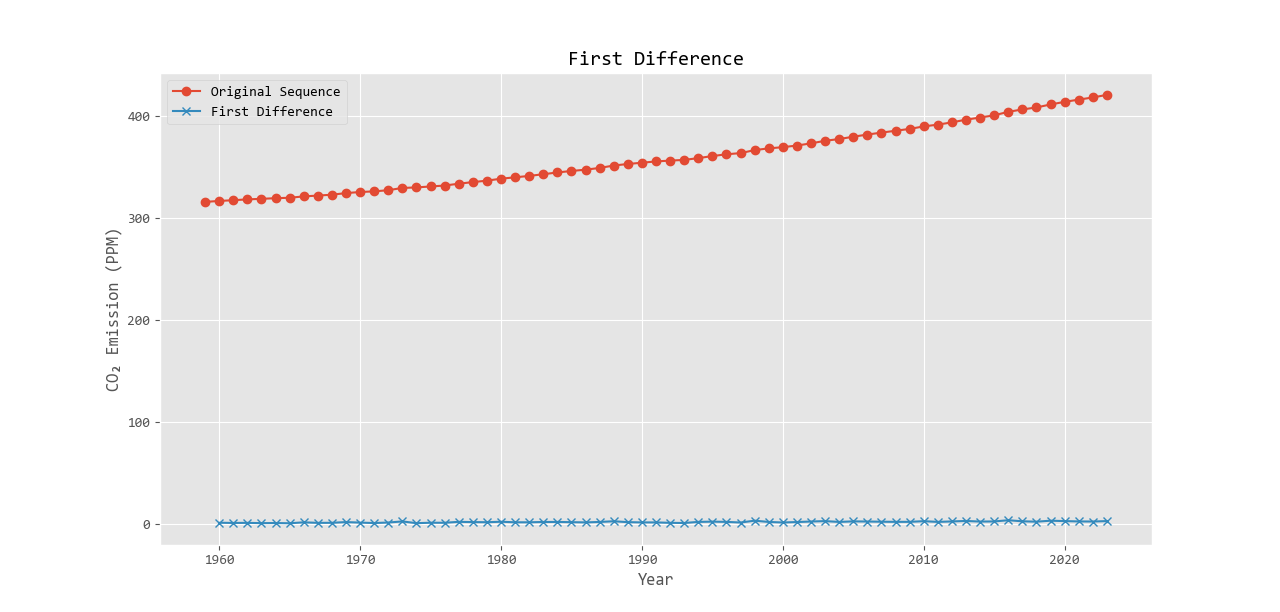
\includegraphics[width=1\linewidth]{img/First Difference.png}
        \caption{First Difference}
        \label{first_diff}
    \end{figure}
    
    \subsubsection*{STEP 2}

    Then we need to determine the order of the AR and MA parts of the model, i.e. the value of $p$ and $q$. We can use the autocorrelation function (ACF) and partial autocorrelation function (PACF) to do this.
    
    ACF, as the name suggests, measures the correlation between the time series and its lag, which then helps us to identify the order of the MA part of the model. PACF, on the other hand, measures the correlation between the time series and its lag, but it does this after removing the variations already explained by the intervening comparisons. This helps us to identify the order of the AR part of the model. The ACF and PACF graphs are plotted in \hyperref[acf]{Figure \ref*{acf}}.

    \begin{figure}[htbp]
        \centering
        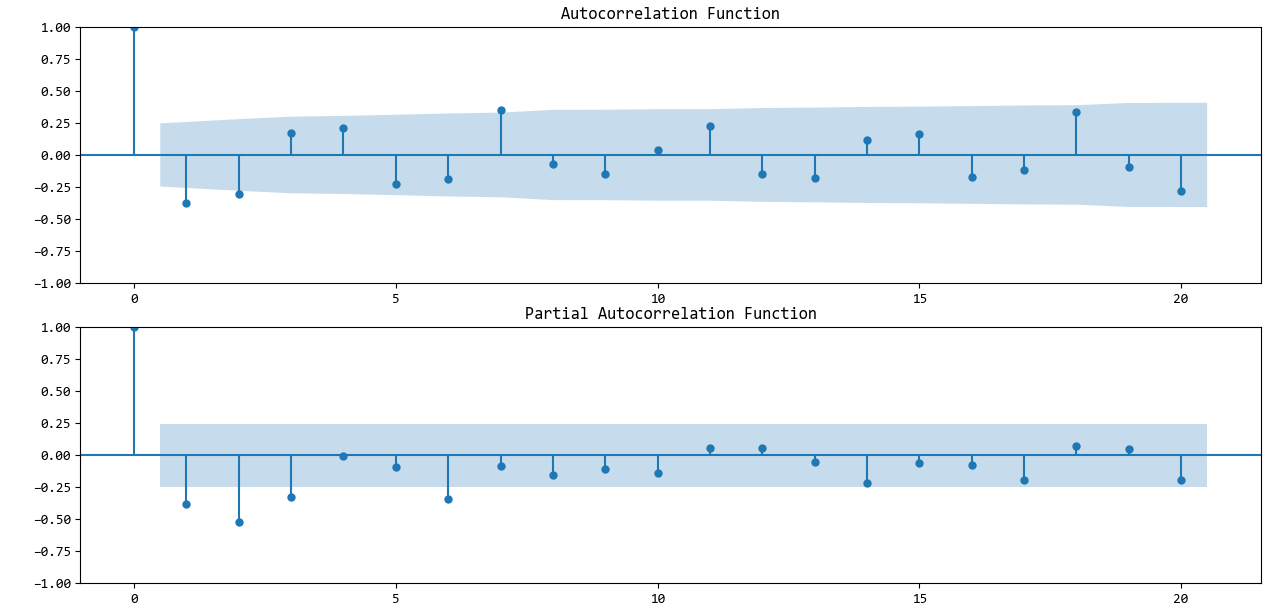
\includegraphics[width=1\linewidth]{img/acf.png}
        \caption{ACF \& PACF}
        \label{acf}
    \end{figure}

    Combining the ACF and PACF graphs, we can take $p=3$ and $q=2$ in our ARIMA model.

    \subsubsection*{STEP 3}
    Since we have already determined our model to be ARIMA$(3,1,2)$, we only need to determine the value of coefficients in \hyperref[6]{Equation 6}, which can be achieved simply by solving a system of linear equations based on the existing data points. The final prediction result is displayed in \hyperref[arima]{Figure \ref*{arima}}, with predicted ppm value in year $2030,2050,2070,2100$ being $437.57,483.18,526.65,588.04$ respectively.

    \begin{figure}[htbp]
        \centering
        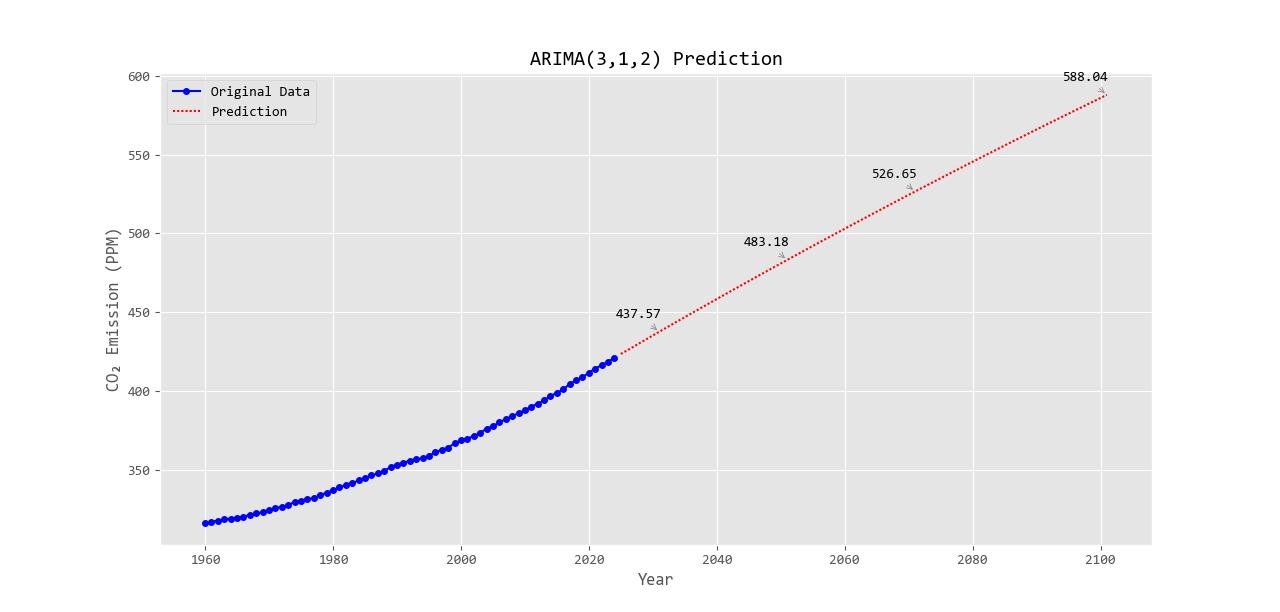
\includegraphics[width=1\linewidth]{img/arima.png}
        \caption{ARIMA$(3,1,2)$ Prediction}
        \label{arima}
    \end{figure}

    \subsection{Results and Analysis}
    
    To conclude, I combine the results from polynomial fitting and ARIMA model together, as shown in \hyperref[arima]{Figure \ref*{combination}}, and the compared value in specific years (2030, 2050, 2070, 2100) are shown in \hyperref[yearpred]{Table \ref*{yearpred}}.

    The graph shows that all four predictions report considerable increase in \ce{CO2} emission in the few decades, which is consistent with the general trend of the data point. We also notice that ARIMA model and linear fitting are more stable than quadratic and cubic fitting. Since the ARIMA model can capture the time dependency of the data, it is more accurate than polynomial fitting.

    \begin{figure}[htbp]
        \centering
        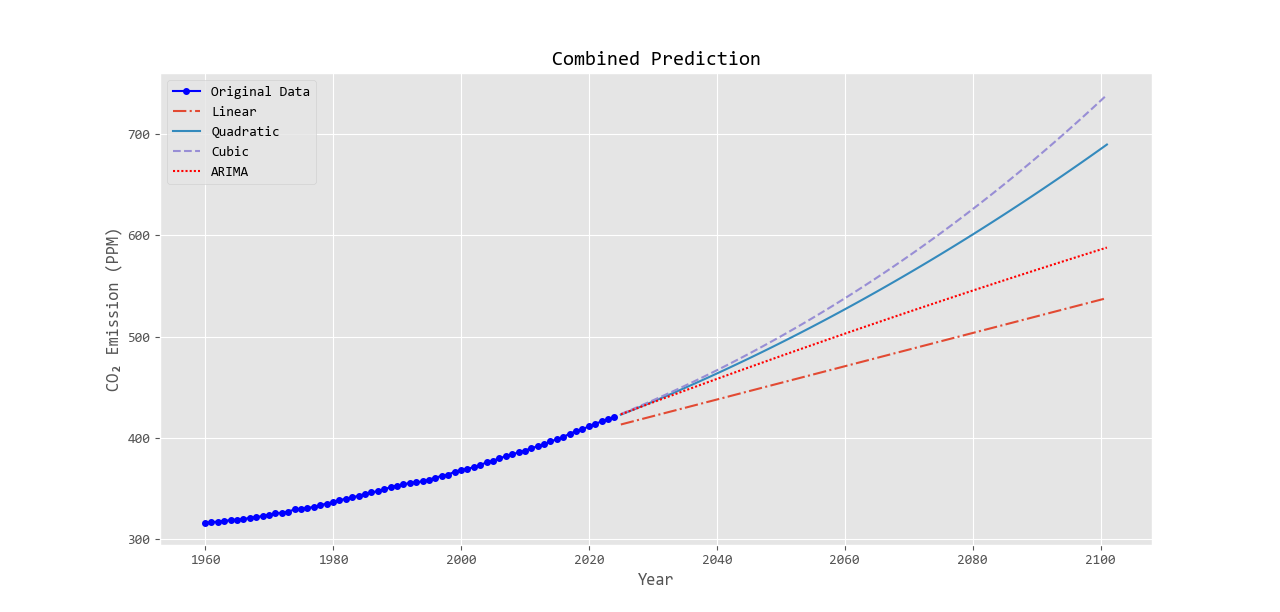
\includegraphics[width=1\linewidth]{img/combination.png}
        \caption{Combined Prediction}
        \label{combination}
    \end{figure}
    
    \begin{table}[htbp]
    \renewcommand*{\arraystretch}{1.3}
    \centering
    \caption{Specific Year Prediction}
    \begin{tabular}{ccccc}
        \toprule[2pt]
        Year&Linear&Quadratic&  Cubic&  ARIMA\\
        \midrule
        2030&423.28&438.64&  440.02&  437.57\\
        2050&456.11&497.23&  503.94&  483.18\\
        2070&488.94&566.32&  584.04&  526.65\\
        2100&538.18&689.68&  738.70&  588.04\\
        \bottomrule[2pt]
    \end{tabular}
    \label{yearpred}
    \end{table}

    It's worth mentioning that our prediction is quite different from the prediction made by OECD in 2012, which predicts the \ce{CO2} emission to reach 685 ppm by 2050, as previously mentioned in literature review \autocite{organisation_for_economic_co-operations_and_development_oecd_2012}. The difference may be due to people's awareness of global warming and the effort to reduce \ce{CO2} emission currently. However, we should recognize that the emission condition is still not optimistic, and current effort is not enough to stop the global warming, as the \ce{CO2} emission is still increasing stably. Therefore, we should continue to take actions and make effort to reduce \ce{CO2} emission, in order to protect our environment and the earth.

    \section{Relationship}
    \subsection{Introduction}
    
    Global warming is a serious issue that is affecting the world. It is a result of the increase in the Earth's average surface temperature due to the release of greenhouse gases. These gases trap heat in the atmosphere, causing the Earth to warm up. This warming has led to a number of negative effects, including rising sea levels, extreme weather events, and loss of biodiversity. As a typical kind of greenhouse gas, \ce{CO2} is widely considered as the main culprit of global warming. And as we plot the temperature and \ce{CO2} emission together in \hyperref[co2_temp]{Figure \ref*{co2_temp}}, we can see that the general trend of the temperature basically matches that of the \ce{CO2} emission. However, to what extent does \ce{CO2} emission contribute to global warming? I will use covariance and build a linear regression model to give a specific answer to this question.
    
    \begin{figure}[htbp]
        \centering
        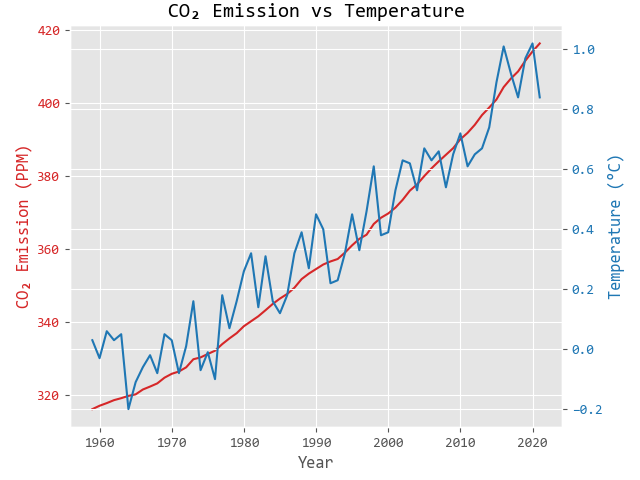
\includegraphics[width=0.5\linewidth]{img/co2_temp.png}
        \caption{\ce{CO2} Emission VS Temperature}
        \label{co2_temp}
    \end{figure}
    
    \subsection{Methodology}
    \subsubsection{Covariance}
    Covariance is a statistic tool which measure the joint variability, or the degree of relationship between two random variables \autocite{rice_mathematical_2007}. This function directly shows how two variables change together. Specifically, when one variable changes, another variable change in the same sign or direction, then they are considered to have a positive covariance. On the contrary, if they change in the opposite direction, then they have a negative covariance. However, if one's change does not affect the other, then we say they have a covariance of zero, in other words, they are independent. The magnitude of the covariance indicates the strength of the relationship between the two variables. The larger the covariance, the stronger the relationship. 
    
    As for its formula, the covariance of two random variables $X$ and $Y$ is defined as:
    
    \begin{equation}
        \begin{aligned}
        \operatorname{Cov}(X, Y)&=E[(X-E[X])(Y-E[Y])] \\
        &=E[XY]-E[X]E[Y]
        \end{aligned}
    \end{equation}
    
    Therefore, in order to find the relationship between \ce{CO2} and global warming, we just need to calculate the covariance between the temperature and \ce{CO2} emission by simply substituting the data into the formula. 

    The calculation is trivial and our result is $9.333$. However, the matter is that we cannot draw any conclusion simply from the number because the number itself has no meaning or implication since we do not know whether the result to be large or small. Therefore, a solution to this problem is to restrict the covariance to a range of $[-1,1]$ so that the result can be interpreted. This can be done by normalizing the variables before calculating the covariance. We use the Z-score normalization here, which is a common method to normalize the data. For example, for a random variable $X$, the normalized value is obtained by:
    
    \begin{equation}
        X^*=\frac{X-\mu_X}{\sigma_X}
    \end{equation} where $\mu_X$ is their mean and $\sigma_X$ is their standard deviation. Then we can calculate the covariance of the normalized variables. 
    
    Our final result is $0.977$, which is very close to $1$. This means that the temperature and \ce{CO2} emission have a strong positive relationship. In other words, the increase in \ce{CO2} emission is highly likely to lead to the increase in temperature. This result is consistent with the general understanding of global warming.

    \subsubsection{Linear Regression}
    We have used covariance to prove the positive relationship between  \ce{CO_2} emission and global warming. However, there are some limitations of covariance such as the sensitivity to outliers. Therefore, we use linear regression model to examine the relationship.

    Linear Regression is a statistical method that models the relationship between two variables by fitting a linear equation to the observed data. It is similar to the linear fitting method we used previously to predict the future \ce{CO2} emission. However, our aim here is to describe the relationship between \ce{CO2} emission and global warming by finding the best-fit line, not for prediction. The formula of the linear regression model is given by:

    \begin{equation}\label{9}
        f(x)=\beta_0+\beta_1x+\varepsilon
    \end{equation} where $\beta_0$ is the intercept, $\beta_1$ is the slope, $x$ is the independent variable, and $\epsilon$ is the error term. The error term represents the difference between the observed value and the predicted value. Similarly, our goal is to find the best-fit line that minimizes the sum of the squared errors.

    For preparation, we first plot the graph between \ce{CO2} and temperature in \hyperref[scatter_temp]{Figure \ref*{scatter_temp}}, where the emission of \ce{CO2} is considered to be the independent variable since we believe that the increase in \ce{CO2} emission leads to the increase in temperature. 

    \begin{figure}[htbp]
        \centering
        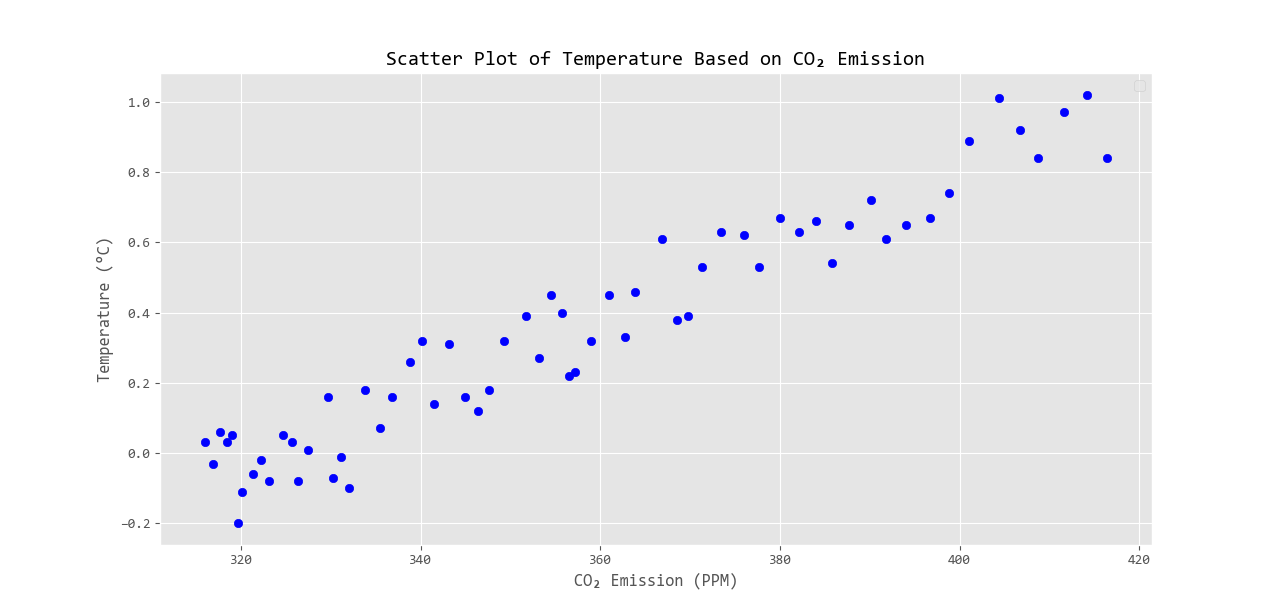
\includegraphics[width=1\linewidth]{img/scatter temp.png}
        \caption{Scatter Plot of Temperature Based on \ce{CO2} Emission}
        \label{scatter_temp}
    \end{figure}

    Based on that, we can easily calculate the slope and intercept of the best-fit line, which is
    
    \begin{equation}\label{10}
        f(x)=0.0105x-3.393
    \end{equation}
    
    \begin{figure}[htbp]
        \centering
        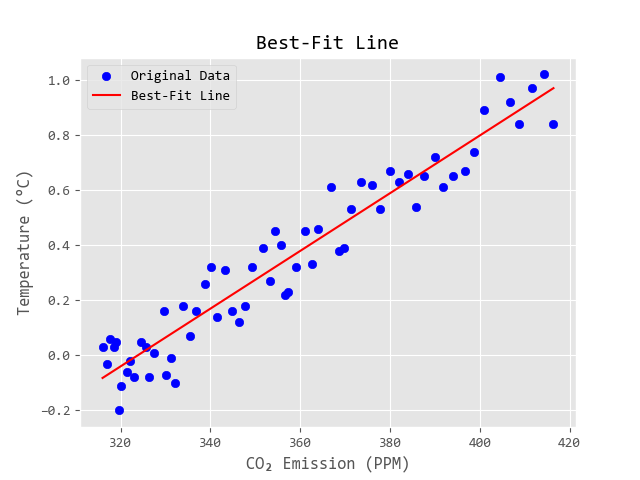
\includegraphics[width=0.5\linewidth]{img/best-fit line.png}
        \caption{Best-Fit Line}
        \label{bestfit}
    \end{figure}
    
    The corresponding graph is shown in \hyperref[bestfit]{Figure \ref*{bestfit}}.

    Furthermore, we need to use several methods to evaluate the performance of the model, that means, we need to check the reliability of our result that temperature is linearly correlated to \ce{CO2} emission with \hyperref[10]{Equation 10} to be their exact relationship.

    Firstly, we try to scatter the residual errors, i.e. $\varepsilon$ in \hyperref[9]{Equation 9}, to see the range of the errors and the randomness of the errors. As shown in \hyperref[residual]{Figure \ref*{residual}}, we can clearly observe that the errors are randomly distributed around zero within a fairly small range, which indicates that the linear regression model is unbaised and appropriate for the data.

    \begin{figure}[htbp]
        \centering
        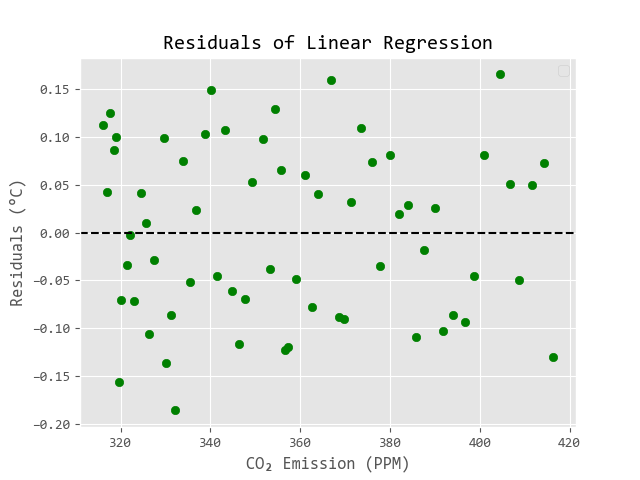
\includegraphics[width=0.5\linewidth]{img/residual.png}
        \caption{Residual Graph}
        \label{residual}
    \end{figure}

    We then want to evaluate the model by some common metrics, including Mean Absolute Error (MAE), Mean Square Error (MSE), Root Mean Square Error (RMSE), Mean Absolute Percentage Error (MAPE), all of which shows the degree of errors by further handle the residuals. And lower values of these metrics indicate a better model. The results are shown in \hyperref[errorsta]{Table \ref*{errorsta}}.

    \begin{table}[htbp]
    \renewcommand*{\arraystretch}{1.3}
    \centering
    \caption{Error Statistics}
    \begin{tabular}{ccccc}
        \toprule[2pt]
        MAE&MSE&RMSE&MAPE\\
        \midrule
        0.0786&0.00790&0.0889&69.2\%\\
        \bottomrule[2pt]
    \end{tabular}
    \label{errorsta}
    \end{table}

    These metrics are intuitively really small, which means the model is quite reliable. However, they range from $[0,\infty)$, which means they are based on non-normalized data and are not comparable. Therefore, we introduce the method of $R^2$, or the coefficient of determination, which is a normalized metric that ranges from $[0,1]$. 

    The $R^2$ metric is a typical statistical measure used in the context of predictive modeling and regression analysis to assess the goodness of fit of a model. It provides a measure of how well observed outcomes are replicated by the model, based on the proportion of total variation of outcomes explained by the model. A higher $R^2$ value means that the model fits the data better. Mathematically, $R^2$ value is defined by
    
    \begin{equation}
        R^2=1-\frac{\sum_{i=1}^{n}(y_i-\hat{y}_i)^2}{\sum_{i=1}^{n}(y_i-\bar{y})^2}
    \end{equation}
    
    Our finally obtained value is $R^2=0.924$, which is quite close to 1. Therefore, based on the above few metrics, we can conclude that the linear regression model is quite reliable and the relationship between \ce{CO2} emission and global warming is nearly linearly correlated.

    \subsection{Results and Analysis}
    In conclusion, we have developed two methods to answer the question of how significantly emissions of carbon dioxide impact on global warming. For the first method, we have used the covariance to measure the relationship between the two variables. In order to make our result interpretable, we find the covariance based on the normalized data. The covariance value we obtained is above $95\%$, so we can basically regard \ce{CO2} and the temperature to be closely related. This method is simple and intuitive, but it is not very accurate, for it is sensitive to high volatility and outliers. 

    Then we consider the linear regression model, which is also a typical method to measure the relationship between two variables. We have found the best-fit line for the Temperature-\ce{CO2} data points in \hyperref[10]{Equation 10}. The linear regression model is more accurate than the covariance method, and it is also more robust, and it further provides us with the exact form of their relationship. However, we should recogize the drawbacks of this model such as the assumption it bases on that two variables are linearly related. Then we plotted their residuals and used some metrics including MAE, MSE, RMSE, MAPE to examine the reliablity of the linear regression model. We also used the $R^2$ metric to evaluate the model, which has great advantages including its high interpretability for us to draw conclusions and its standardized and scale-free measure it provides. Combining the results of these evalutions we can conclude that the linear regression model is quite an appropriate method to measure and model the relationship between \ce{CO2} emission and global warming.

    From all these conclusions above we can infer that \ce{CO2} is strongly contributing to the increase of temperature, and they have a linear relationship for the most part. Therefore, we should increase the awareness of reducing \ce{CO2} emission to mitigate global warming and its adverse effects.

    \section{Discussion}
    \subsection{Introduction}
    Recall that the topic of our research is \textit{How does carbon dioxide affect human's life}. Based on this topic, in the literature review part, I qualitatively investigate from previous researches the \ce{CO2} emission condition, its impact on the ecosystem and human beings, and human's current responses to dealing this issue. Then I focus on the prediction of \ce{CO2} emission and the relationship between \ce{CO2} and global warming in the next two sections, where I build several models to quantitatively analyze these problems, so as to provide a comprehensive understanding of the impact of \ce{CO2} on human's life, aiming at reflecting the current situation and predicting the future trend of \ce{CO2} emission, which may help to guide the future policy-making and human's actions. In this section, I will discuss and summarize the implications and limitations of my results, and provide some suggestions for future researches.
    
    \subsection{Implications}
    This report explores detailedly the effect of the \ce{CO2} to global warming and the general trend of \ce{CO2} emission. Firstly, we make our predictions to the future \ce{CO2} emission through polynomial fitting and ARIMA models, and the combined result is shown in \hyperref[combination]{Figure \ref*{combination}} and \hyperref[yearpred]{Table \ref*{yearpred}}. Through what we have found, we can conclude that the \ce{CO2} emission will continue increasing steadily in the future few decades, and will reach a shocking value of roughly $600$ to $700$ PPM in year $2100$. Generally speaking, this provides valuable insights into the potential trajectory of global warming. By quantifying these trends, it emphasizes the urgent need for robust, actionable strategies to mitigate \ce{CO2} emissions. 

    Secondly, by methods of covariance and linear regression, we have established a clear, quantifiable relationship between \ce{CO2} emissions and global warming, reinforcing the concept that rising \ce{CO2} levels significantly contribute to temperature increases. This finding can serve as an evidence to support the rationale for international agreements aimed at reducing greenhouse gas emissions.

    In terms of policies and dicision-making in real life, this study provides a data-driven foundation for policymakers to draft, implement, and adjust environmental policies. By offering a clearer understanding of the potential future scenarios of climate change, this research aids in the formulation of more effective, long-term strategies for emissions reduction, climate adaptation, and sustainability efforts.
    
    \subsection{Limitations}
    This research, while comprehensive in its attempt to quantify the effects of \ce{CO2} emissions on global warming and predict future trends, acknowledges several limitations that must be considered when interpreting the findings.

    \subsubsection*{Data and Methodological Constraints}
    The predictions of future \ce{CO2} emissions and their effects on global warming are primarily based on polynomial fitting and ARIMA models. While these methods are robust for the analysis conducted, they inherently assume that past trends and patterns will continue into the future. This assumption may not account for unpredictable changes in global policies, technological advancements, human behaviors, and natural climate variations, which can significantly alter future emission trajectories and climate responses.

    \subsubsection*{Scope of the Study}
    The research focuses on \ce{CO2} emissions without extensively considering other greenhouse gases and pollutants that contribute to global warming and climate change. Consequently, the study's conclusions may not fully encapsulate the broader context of anthropogenic climate change, overlooking the synergistic effects of multiple emission sources.

    \subsubsection*{Temporal Constraints}
    The study's predictive models are constrained by the historical data available, covering a limited time frame. The reliability of long-term forecasts is inherently uncertain, as they do not account for future socio-economic changes, policy interventions, and technological innovations that could significantly impact \ce{CO2} emission patterns.
    
    \subsubsection*{Model Simplifications}
    To maintain tractability, the models employed in this study simplify complex climate processes and interactions. These simplifications may not fully capture the dynamic and nonlinear nature of the climate system, potentially underestimating or overestimating the impact of \ce{CO2} emissions on global warming.

    \subsubsection*{Potential for Overfitting}
    In employing polynomial fitting and ARIMA models for prediction, there is a risk of overfitting, where models may too closely align with the historical data, compromising their predictive accuracy for future trends.
    
    \subsection{Future Recommendations}
    To further investigate in this field, I have several recommendations for future studies. 
    
    Firstly, to do more accurate predictions, I think future research should strive to develop more advanced model techniques such as machine learning or neural network which this project does not involve. Alternatively, future researchers can also make an effort to collect more accurate data in a wider range of years which the models are based on. 

    Moreover, future researchers can also try to integrate more comprehensive datasets that encompass a wider array of variables influencing global warming such as \ce{CH4} or \ce{N2O}. They can carry out a comparison among pollutants to help identify comprehensive roles the greenhouse gas contributes to global warming.

    \subsection{Conclusion}    
    In conclusion, this project comprehensively analyzes the influence of \ce{CO2} on human beings, and we concretely make an effort to predict the future \ce{CO2} emission and find the relationship between \ce{CO2} and global warming. Though a few limitations, I think my research is generally satisfying and it lays a groundwork for future investigation, and I hope my research can help rise people's awareness to reduce \ce{CO2} emissions to control global warming, by which we make an effort to protect the earth and forge a sustainable future.
    
    \newpage
    \section{Bibliography}
    \printbibliography[heading=none]
    
\end{document}